\documentclass{beamer}

\mode<presentation>
{
  \usetheme{Darmstadt}
  \usecolortheme{beaver}
  \usefonttheme{serif}
  \setbeamertemplate{navigation symbols}{}
  \setbeamertemplate{caption}[numbered]
}

\usepackage[english]{babel}
\usepackage[utf8]{inputenc}
\usepackage{booktabs}
\usepackage{amsmath}
\usepackage{graphicx}
\usepackage{tikz}
\usetikzlibrary{positioning, decorations.pathreplacing, calc}
\graphicspath{{figs/}}

\title[Multi-Task ViT]{Multi-Task Learning with Vision Transformers:\\Joint Classification and Saliency Prediction}
\author{Nicholas Welsh}
\institute{Florida Institute of Technology\\Department of Computer Science \& Mathematics}
\date{March 2026}

\begin{document}

\begin{frame}
  \titlepage
\end{frame}

\begin{frame}{Outline}
  \tableofcontents
\end{frame}

% ============================================================
\section{Motivation}
% ============================================================

\begin{frame}{From Classical ML to Deep Learning}
\begin{itemize}
  \item So far we have seen models like KNN, decision trees, and logistic regression.
  \item These work well on \textbf{structured, tabular data} (spreadsheets with rows and columns).
  \item But images are not tables. A $224\!\times\!224$ color image has over 150,000 raw pixel values. Classical models struggle with this.
  \item \textbf{Neural networks} solve this by automatically learning which patterns in those pixels matter, instead of us hand-picking features.
\end{itemize}
\vfill
\textbf{This project:} we use a neural network called a Vision Transformer to process images directly.
\end{frame}

\begin{frame}{What Is a Neural Network?}
\begin{columns}
\column{0.55\textwidth}
\begin{itemize}
  \item Made of layers of simple units (``neurons'') connected together.
  \item Each layer transforms its input and passes it to the next.
  \item Early layers detect simple patterns (edges, colors). Later layers combine them into complex ones (eyes, objects).
  \item A \textbf{deep} network has many layers, so it can learn very complex patterns.
\end{itemize}
\column{0.45\textwidth}
\begin{center}
\resizebox{0.95\columnwidth}{!}{%
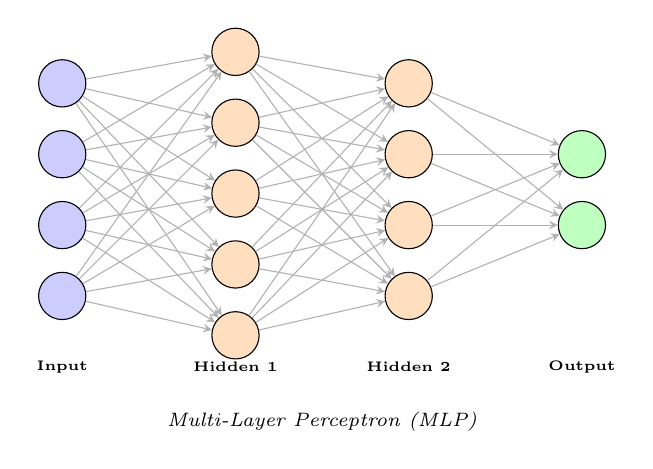
\begin{tikzpicture}[
  neuron/.style={circle, draw, minimum size=0.6cm, inner sep=0pt, fill=#1},
  neuron/.default={white},
  >=stealth
]
  % input layer
  \foreach \i in {1,...,4} {
    \node[neuron=blue!20] (i\i) at (0, -\i*0.9+0.5) {};
  }
  % hidden layer 1
  \foreach \j in {1,...,5} {
    \node[neuron=orange!25] (h1\j) at (2.2, -\j*0.9+0.9) {};
  }
  % hidden layer 2
  \foreach \k in {1,...,4} {
    \node[neuron=orange!25] (h2\k) at (4.4, -\k*0.9+0.5) {};
  }
  % output layer
  \foreach \o in {1,...,2} {
    \node[neuron=green!25] (o\o) at (6.6, -\o*0.9-0.4) {};
  }
  % connections
  \foreach \i in {1,...,4} {
    \foreach \j in {1,...,5} { \draw[->, gray!60] (i\i) -- (h1\j); }
  }
  \foreach \j in {1,...,5} {
    \foreach \k in {1,...,4} { \draw[->, gray!60] (h1\j) -- (h2\k); }
  }
  \foreach \k in {1,...,4} {
    \foreach \o in {1,...,2} { \draw[->, gray!60] (h2\k) -- (o\o); }
  }
  % labels below each column at fixed y
  \node[font=\tiny\bfseries] at (0, -4.0) {Input};
  \node[font=\tiny\bfseries] at (2.2, -4.0) {Hidden 1};
  \node[font=\tiny\bfseries] at (4.4, -4.0) {Hidden 2};
  \node[font=\tiny\bfseries] at (6.6, -4.0) {Output};
  % caption
  \node[font=\scriptsize\itshape] at (3.3, -4.7)
    {Multi-Layer Perceptron (MLP)};
\end{tikzpicture}%
}
\end{center}
\end{columns}
\end{frame}

\begin{frame}{What Is a Vision Transformer?}
\small
\begin{columns}[c]
\column{0.50\textwidth}
\begin{itemize}
  \item A \textbf{Vision Transformer (ViT)} is a neural network for images.
  \item Instead of a sliding window, it:
  \begin{enumerate}
    \item Cuts the image into a grid of \textbf{patches}.
    \item Processes all patches at once.
  \end{enumerate}
  \item \textbf{Attention} lets the model decide which patches matter.
  \item We use \textbf{DeiT-Small} (Data-efficient Image Transformer), pretrained on 1.2M images.
\end{itemize}
\column{0.50\textwidth}
\begin{center}
\resizebox{0.85\columnwidth}{!}{%
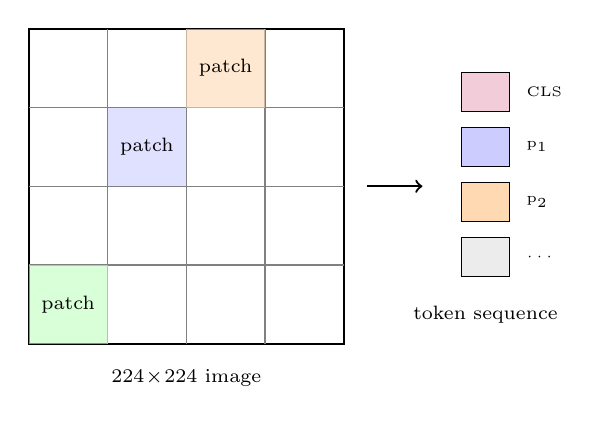
\begin{tikzpicture}
  % image grid
  \draw[thick] (0,0) rectangle (4,4);
  % grid lines (4x4 for visual clarity, represents 14x14)
  \foreach \x in {1,2,3} {
    \draw[gray] (\x,0) -- (\x,4);
    \draw[gray] (0,\x) -- (4,\x);
  }
  % highlight a few patches
  \fill[blue!20, opacity=0.6] (1,2) rectangle (2,3);
  \fill[orange!30, opacity=0.6] (2,3) rectangle (3,4);
  \fill[green!25, opacity=0.6] (0,0) rectangle (1,1);
  % labels
  \node[font=\scriptsize] at (1.5, 2.5) {patch};
  \node[font=\scriptsize] at (2.5, 3.5) {patch};
  \node[font=\scriptsize] at (0.5, 0.5) {patch};
  % arrow to sequence
  \draw[->, thick] (4.3, 2) -- (5.0, 2);
  % token sequence
  \foreach \i/\c in {0/purple!20, 1/blue!20, 2/orange!30, 3/gray!15} {
    \node[draw, fill=\c, minimum width=0.6cm, minimum height=0.5cm, font=\tiny] at (5.8, 3.2-\i*0.7) {};
  }
  \node[font=\tiny, right] at (6.2, 3.2) {CLS};
  \node[font=\tiny, right] at (6.2, 2.5) {p$_1$};
  \node[font=\tiny, right] at (6.2, 1.8) {p$_2$};
  \node[font=\tiny, right] at (6.2, 1.1) {$\cdots$};
  \node[font=\scriptsize, below] at (2, -0.2) {$224\!\times\!224$ image};
  \node[font=\scriptsize, below] at (5.8, 0.6) {token sequence};
\end{tikzpicture}%
}
\end{center}
\end{columns}
\end{frame}

\begin{frame}{Why Multi-Task Learning?}
\begin{itemize}
  \item Most models do one thing: ``Is this a dog?''
  \item \textbf{Multi-task learning} trains one model to do multiple things at once.
  \item Related tasks share useful patterns, so learning one can help the other.
  \item Benefits: more efficient (one model, not two) and can improve accuracy through shared features.
\end{itemize}
\vfill
\begin{center}
  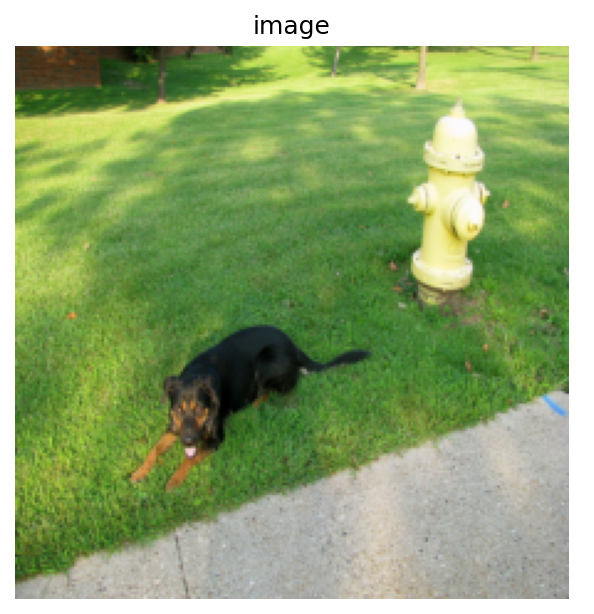
\includegraphics[height=3cm]{dog_original.png}
\end{center}
\vspace{-0.2cm}
\begin{center}
{\small\ttfamily \{"labels": ["dog", "fire\_hydrant"], "saliency": "14x14 heatmap"\}}
\end{center}
\end{frame}

% ============================================================
\section{Model}
% ============================================================

\begin{frame}{Our Two Tasks}
\begin{columns}
\column{0.5\textwidth}
\textbf{Task 1: Classification}
\begin{itemize}
  \item ``What objects are in this image?''
  \item Labels: 20 common categories (person, dog, car, etc.)
  \item An image can contain multiple objects (multi-label).
\end{itemize}

\column{0.5\textwidth}
\textbf{Task 2: Saliency Prediction}
\begin{itemize}
  \item ``Where do humans look in this image?''
  \item Ground truth: actual gaze data from thousands of people.
  \item Output: a heatmap showing predicted gaze density.
\end{itemize}
\end{columns}
\end{frame}

\begin{frame}{How the Model Works}
\begin{center}
\resizebox{0.85\linewidth}{!}{%
  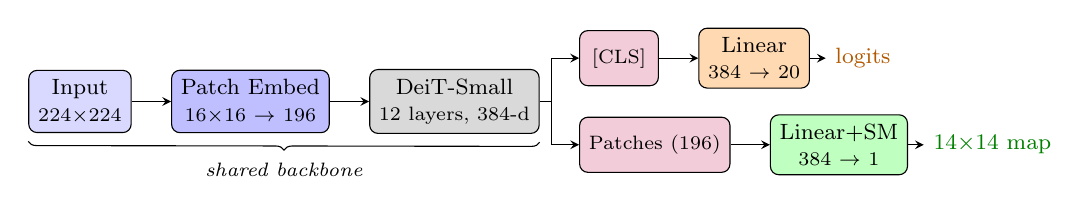
\begin{tikzpicture}[
    node distance=0.5cm,
    box/.style={draw, rounded corners=3pt, minimum height=0.7cm, align=center, font=\footnotesize},
    >=stealth
  ]
    \node[box, fill=blue!15, minimum width=1.3cm] (img)
      {Input\\\scriptsize 224$\times$224};
    \node[box, fill=blue!25, minimum width=1.4cm, right=of img] (patch)
      {Patch Embed\\\scriptsize 16$\times$16 $\to$ 196};
    \node[box, fill=gray!30, minimum width=1.7cm, right=of patch] (backbone)
      {DeiT-Small\\\scriptsize 12 layers, 384-d};
    \node[box, fill=purple!20, minimum width=1.0cm, above right=0.55cm and 0.5cm of backbone.east, anchor=west] (cls)
      {\scriptsize [CLS]};
    \node[box, fill=purple!20, minimum width=1.0cm, below right=0.55cm and 0.5cm of backbone.east, anchor=west] (ptok)
      {\scriptsize Patches (196)};
    \node[box, fill=orange!30, minimum width=1.3cm, right=of cls] (clshead)
      {Linear\\\scriptsize 384 $\to$ 20};
    \node[box, fill=green!25, minimum width=1.3cm, right=of ptok] (salhead)
      {Linear+SM\\\scriptsize 384 $\to$ 1};
    \node[right=0.2cm of clshead, font=\footnotesize, text=orange!70!black] (clsout) {logits};
    \node[right=0.2cm of salhead, font=\footnotesize, text=green!50!black] (salout) {14$\times$14 map};
    \draw[->] (img) -- (patch);
    \draw[->] (patch) -- (backbone);
    \draw[->] (backbone.east) -- ++(0.15,0) |- (cls.west);
    \draw[->] (backbone.east) -- ++(0.15,0) |- (ptok.west);
    \draw[->] (cls) -- (clshead);
    \draw[->] (ptok) -- (salhead);
    \draw[->] (clshead) -- (clsout);
    \draw[->] (salhead) -- (salout);
    \draw[decorate, decoration={brace, amplitude=3pt, mirror}]
      ([yshift=-3pt]img.south west) -- ([yshift=-3pt]backbone.south east)
      node[midway, below=4pt, font=\scriptsize\itshape] {shared backbone};
  \end{tikzpicture}%
}
\end{center}
\begin{itemize}
  \item The image is split into 196 patches ($14 \times 14$ grid).
  \item All patches are processed together by the transformer backbone.
  \item Two separate ``heads'' read the output:
  \begin{itemize}
    \item \textbf{Classification head:} looks at a summary token (CLS) $\rightarrow$ predicts object categories.
    \item \textbf{Saliency head:} looks at each patch $\rightarrow$ predicts how likely people are to look there.
  \end{itemize}
\end{itemize}
\end{frame}

\begin{frame}{What Is Fine-Tuning?}
\begin{itemize}
  \item DeiT-Small was already trained on 1.2 million images to recognize 1,000 object types.
  \item It already ``knows'' how to see edges, textures, shapes, and objects.
  \item Instead of training from scratch, we \textbf{fine-tune}: we take this pretrained model and continue training it on our specific data.
  \item This is much faster and works better than starting from zero, especially when we have limited data (10,000 images).
\end{itemize}
\vfill
\textbf{Analogy:} teaching someone who already speaks English to read medical papers is easier than teaching someone who has never seen text.
\end{frame}

% ============================================================
\section{Data}
% ============================================================

\begin{frame}{Our Datasets}
\begin{itemize}
  \item \textbf{SALICON}: 10,000 training images + 5,000 validation images from COCO.
  \begin{itemize}
    \item Each image comes with a \textbf{fixation map}: a heatmap showing where thousands of people looked.
    \item Collected by tracking mouse movements (approximates eye tracking).
  \end{itemize}
  \item \textbf{COCO 2014}: the same images, but with labels for what objects are present (person, dog, car, etc.).
  \item By pairing these two datasets, each image has both:
  \begin{itemize}
    \item Category labels (``dog, person'') for classification.
    \item A gaze heatmap for saliency prediction.
  \end{itemize}
\end{itemize}
\end{frame}

\begin{frame}{What the Data Looks Like}
\begin{center}
  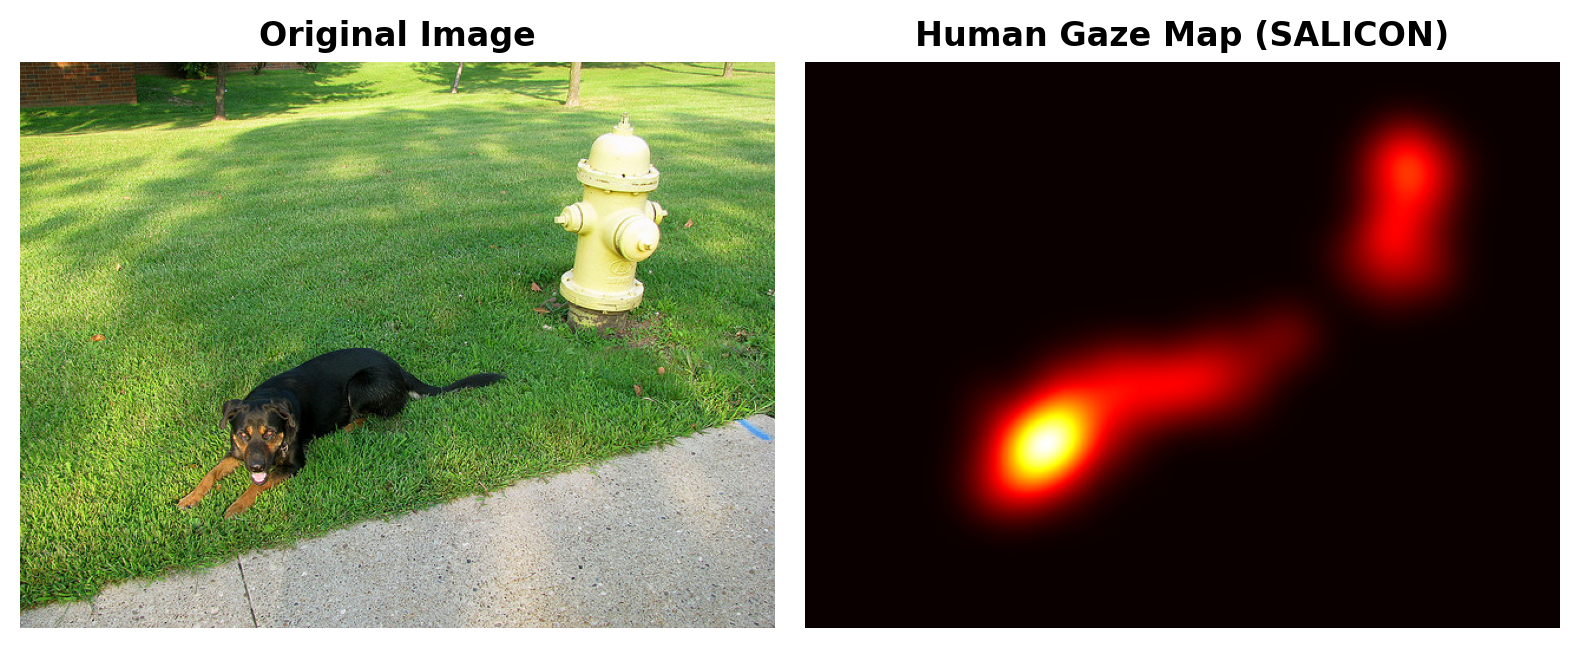
\includegraphics[width=0.95\linewidth]{data_example.png}
\end{center}
\vfill
\small Left: the original photo. Right: the \textbf{SALICON fixation map}, a heatmap showing where thousands of people looked when viewing this image. Bright spots mean more people looked there. This is our ground truth for the saliency task.
\end{frame}

% ============================================================
\section{Experiment}
% ============================================================

\begin{frame}{How We Train the Model}
\begin{itemize}
  \item The model sees each training image and tries to:
  \begin{enumerate}
    \item Predict which objects are present (classification).
    \item Predict where people look (saliency).
  \end{enumerate}
  \item After each prediction, we compute a \textbf{loss}: a number that measures how wrong the model was.
  \item The model adjusts its internal parameters to reduce the loss.
  \item This process repeats for 15 \textbf{epochs} (passes through the full training set).
  \item We save the version of the model that performed best on a held-out validation set.
\end{itemize}
\end{frame}

\begin{frame}{What Is a Loss Function?}
\begin{itemize}
  \item A loss function is how we tell the model ``how wrong you are.''
  \item For classification: \textbf{binary cross-entropy}. Penalizes the model for being confident about wrong labels.
  \item For saliency, we tested two options:
  \begin{itemize}
    \item \textbf{MSE}: average squared difference between prediction and ground truth.
    \item \textbf{KL (Kullback--Leibler) divergence}: measures how different two probability distributions are.
  \end{itemize}
  \item This choice turned out to be the most important design decision in the project.
\end{itemize}
\vfill
\begin{center}
\small
$\mathcal{L} = \underbrace{\text{BCE}(\hat{y},\, y)}_{\text{classification}} + \;\lambda \cdot \underbrace{\mathcal{L}_{\text{sal}}}_{\text{saliency}}$
\qquad
$\mathcal{L}_{\text{sal}} = \begin{cases} \text{MSE}(p,\, \hat{p}) \\ \text{KL}(\,p \;\|\; \hat{p}\,) \end{cases}$
\end{center}
\end{frame}

\begin{frame}{What We Compare Against}
To know if our model is any good, we need baselines:
\vfill
\begin{itemize}
  \item \textbf{Frozen-feature baselines}: use the pretrained model as a fixed feature extractor (no fine-tuning) and train simple classifiers on top.
  \begin{itemize}
    \item Logistic regression (a simple linear classifier)
    \item MLP (a small 1-layer neural network)
  \end{itemize}
  \item \textbf{Single-task ablations}: train with only one task active to see how multi-tasking compares.
  \begin{itemize}
    \item \textbf{cls-only}: only classification, no saliency.
    \item \textbf{sal-only}: only saliency, no classification.
  \end{itemize}
\end{itemize}
\end{frame}

\begin{frame}{How We Measure Success}
\begin{itemize}
  \item \textbf{Classification: mAP} (mean average precision)
  \begin{itemize}
    \item Measures how well the model ranks correct labels above incorrect ones.
    \item 1.0 = perfect, 0.0 = random guessing.
  \end{itemize}
  \item \textbf{Saliency: CC} (correlation coefficient)
  \begin{itemize}
    \item Measures how well the predicted heatmap matches the human gaze heatmap.
    \item 1.0 = perfect match, 0.0 = no relationship.
  \end{itemize}
  \item We also report SIM (distribution overlap) and KL divergence (distributional distance).
\end{itemize}
\end{frame}

% ============================================================
\section{Results}
% ============================================================

\begin{frame}{Training Curves}
\begin{center}
  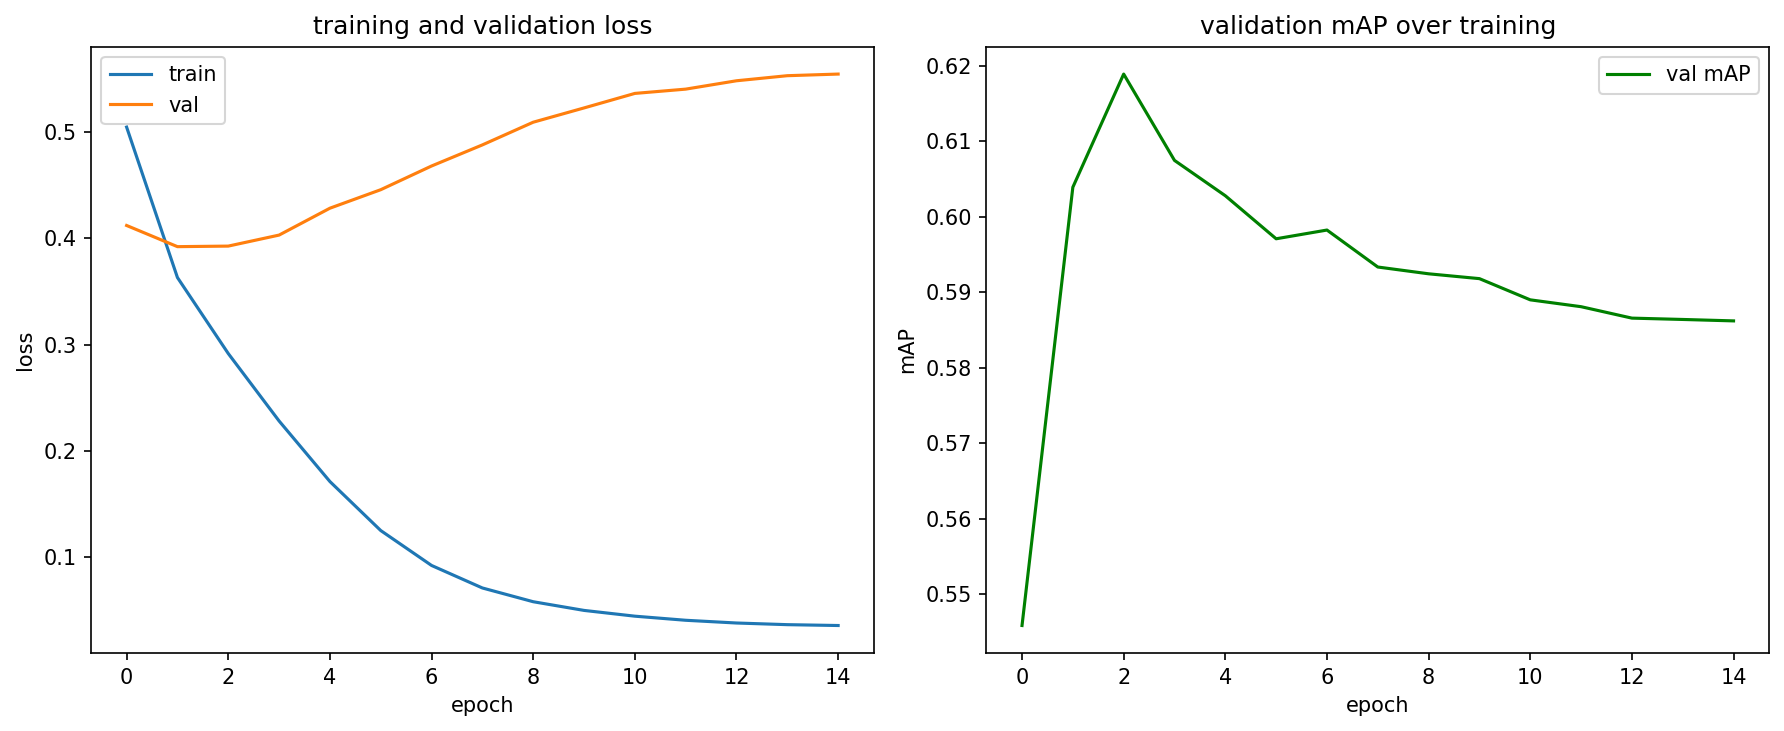
\includegraphics[width=0.9\linewidth]{training_curves_multitask.png}
\end{center}
\begin{itemize}
  \item Left: loss decreases over training (model gets better).
  \item Right: classification accuracy on validation data.
  \item The model peaks early (epoch 2--3), then starts to overfit (memorize training data). We save the best early version.
\end{itemize}
\end{frame}

\begin{frame}{Classification: Fine-Tuning Helps}
\begin{center}
\begin{tabular}{lc}
\toprule
Method & mAP \\
\midrule
Logistic regression (frozen) & 0.556 \\
MLP classifier (frozen) & 0.566 \\
\midrule
ViT cls-only (fine-tuned) & 0.623 \\
ViT multitask (fine-tuned) & 0.604 \\
\bottomrule
\end{tabular}
\end{center}
\vfill
\begin{itemize}
  \item Fine-tuning improves over frozen baselines by 5--6 points.
  \item Multi-task is slightly worse than classification-only (0.604 vs 0.623).
  \item That 1.9-point gap is the ``cost'' of sharing the model with saliency.
\end{itemize}
\end{frame}

\begin{frame}{The Big Surprise: Loss Function Matters More Than Architecture}
\begin{center}
\begin{tabular}{lcccc}
\toprule
Saliency Loss & mAP & CC & SIM & KL \\
\midrule
MSE & 0.612 & 0.196 & 0.430 & 1.087 \\
KL divergence & 0.604 & \textbf{0.899} & \textbf{0.799} & \textbf{0.182} \\
\bottomrule
\end{tabular}
\end{center}
\vfill
\begin{itemize}
  \item Same model, same data, same everything. Only the loss function changed.
  \item Saliency correlation jumps from 0.196 to 0.899.
  \item \textbf{Why?} MSE treats the output as raw numbers. KL divergence treats it as a probability distribution, which is what our model actually outputs.
  \item Lesson: how you measure ``wrongness'' matters as much as the model itself.
\end{itemize}
\end{frame}

\begin{frame}{Visual Comparison}
\begin{center}
  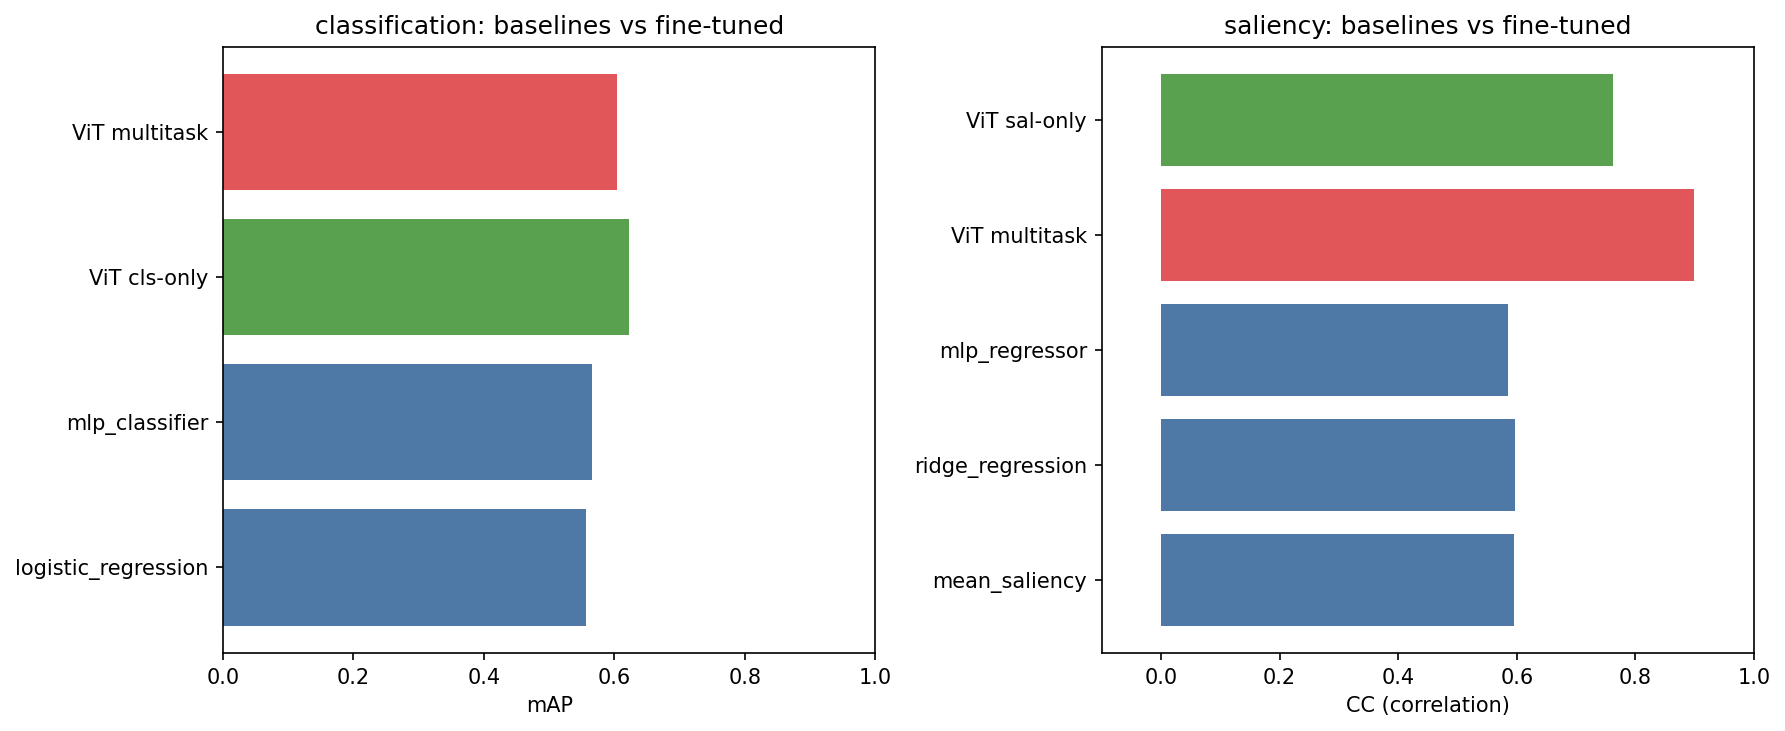
\includegraphics[width=0.9\linewidth]{baseline_comparison.png}
\end{center}
\begin{itemize}
  \item Left: classification accuracy. Fine-tuned models (red/green) beat frozen baselines (blue).
  \item Right: saliency correlation. Fine-tuned models (green) substantially beat baselines (blue).
\end{itemize}
\end{frame}

\begin{frame}{What the Model ``Sees''}
\begin{center}
  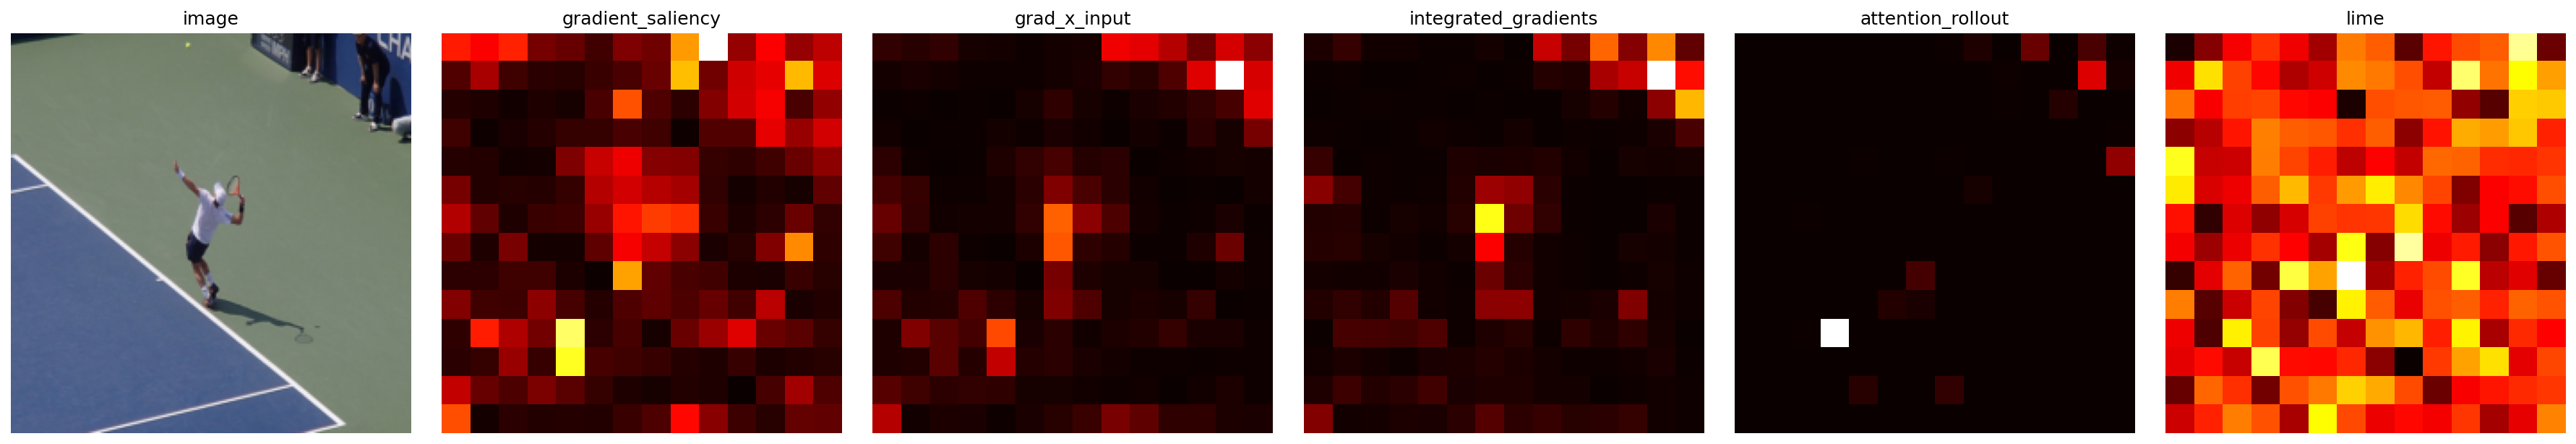
\includegraphics[width=\linewidth]{report_comparison_305.png}
\end{center}
\small A tennis player. The model's saliency head predicts where people look (bright = high attention). The prediction concentrates on the player, matching human gaze patterns.
\end{frame}

% ============================================================
\section{Conclusion}
% ============================================================

\begin{frame}{What We Learned}
\begin{enumerate}
  \item \textbf{One model, two tasks.} A single Vision Transformer can classify images and predict human gaze at the same time, with only a small accuracy trade-off.
  \item \textbf{Fine-tuning beats simple baselines.} Adapting a pretrained model to our data outperforms simpler approaches that use the same model as a fixed feature extractor.
  \item \textbf{Loss function design is critical.} Switching from MSE to KL divergence raised saliency correlation from 0.196 to 0.899 without changing anything else. Choosing the right way to measure error can matter more than choosing the right model.
\end{enumerate}
\end{frame}

\begin{frame}{Why This Matters}
\begin{itemize}
  \item In practice, many real-world problems involve multiple related tasks. Multi-task learning lets you build more efficient systems.
  \item The loss function finding is a cautionary tale: a model can appear to fail when the real problem is how you are training or evaluating it.
  \item Understanding these interactions between model design, loss functions, and evaluation metrics is a core skill in applied machine learning.
\end{itemize}
\end{frame}

\begin{frame}{Limitations}
\begin{itemize}
  \item Results are from a single training run (seed 42). Running multiple times with different random seeds would give more confidence.
  \item KL and MSE losses have different scales, which also changes how the two tasks are balanced. A more thorough study would sweep across different balance settings.
  \item Our saliency maps are low resolution ($14 \times 14$ patches), so they are not directly comparable to high-resolution saliency benchmarks.
\end{itemize}
\end{frame}

\begin{frame}
\begin{center}
\Large\textbf{Questions?}

\vfill
\normalsize
Nicholas Welsh \\
\texttt{nwelsh2024@my.fit.edu} \\
\vspace{0.5cm}
\href{https://github.com/nickvpn/vit-ml-xai-project}{github.com/nickvpn/vit-ml-xai-project}
\end{center}
\end{frame}

\end{document}
